%%%%%%%%%%%%%%%%%%%%%%%%%%%%%%%%%%%%%%%%%
% Beamer Presentation
% LaTeX Template
% Version 1.0 (10/11/12)
%
% This template has been downloaded from:
% http://www.LaTeXTemplates.com
%
% License:
% CC BY-NC-SA 3.0 (http://creativecommons.org/licenses/by-nc-sa/3.0/)
%
%%%%%%%%%%%%%%%%%%%%%%%%%%%%%%%%%%%%%%%%%

%----------------------------------------------------------------------------------------
%	PACKAGES AND THEMES
%----------------------------------------------------------------------------------------

\documentclass{beamer}


\mode<presentation> {

% The Beamer class comes with a number of default slide themes
% which change the colors and layouts of slides. Below this is a list
% of all the themes, uncomment each in turn to see what they look like.

%\usetheme{default}
%\usetheme{AnnArbor}
%\usetheme{Antibes}
%\usetheme{Bergen}
%\usetheme{Berkeley}
%\usetheme{Berlin}
%\usetheme{Boadilla}
\usetheme{CambridgeUS}
%\usetheme{Copenhagen}
%\usetheme{Darmstadt}
%\usetheme{Dresden}
%\usetheme{Frankfurt}
%\usetheme{Goettingen}
%\usetheme{Hannover}
%\usetheme{Ilmenau}
%\usetheme{JuanLesPins}
%\usetheme{Luebeck}
%\usetheme{Madrid}
%\usetheme{Malmoe}
%\usetheme{Marburg}
%\usetheme{Montpellier}
%\usetheme{PaloAlto}
%\usetheme{Pittsburgh}
%\usetheme{Rochester}
%\usetheme{Singapore}
%\usetheme{Szeged}
%\usetheme{Warsaw}

% As well as themes, the Beamer class has a number of color themes
% for any slide theme. Uncomment each of these in turn to see how it
% changes the colors of your current slide theme.

%\usecolortheme{albatross}
%\usecolortheme{beaver}
%\usecolortheme{beetle}
%\usecolortheme{crane}
%\usecolortheme{dolphin}
%\usecolortheme{dove}
%\usecolortheme{fly}
%\usecolortheme{lily}
%\usecolortheme{orchid}
%\usecolortheme{rose}
%\usecolortheme{seagull}
%\usecolortheme{seahorse}
%\usecolortheme{whale}
%\usecolortheme{wolverine}

%\setbeamertemplate{footline} % To remove the footer line in all slides uncomment this line
%\setbeamertemplate{footline}[page number] % To replace the footer line in all slides with a simple slide count uncomment this line

%\setbeamertemplate{navigation symbols}{} % To remove the navigation symbols from the bottom of all slides uncomment this line
}
\usepackage{standalone}
\usepackage{graphicx} % Allows including images
\usepackage{booktabs} % Allows the use of \toprule, \midrule and \bottomrule in tables
\usepackage{tcolorbox}
\usepackage{media9}
\usepackage{float}
\usepackage{tkz-euclide}
\usepackage{amssymb,bm,amsmath}
\newcommand{\norm}[1]{\left\lVert#1\right\rVert}
\renewcommand{\vec}[1]{\ensuremath{\boldsymbol{#1}}}
\newcommand{\mat}[1]{\ensuremath{\boldsymbol{#1}}}
\usetikzlibrary{quotes,angles}
\newcommand{\inputTikZ}[2]{%
     \scalebox{#1}{\input{#2}}
}
\tcbuselibrary{raster}
\tcbuselibrary{fitting}
\definecolor{ku}{RGB}{144,26,30}
\definecolor{ku-yellow}{RGB}{255,249,25}

%----------------------------------------------------------------------------------------
%	TITLE PAGE
%----------------------------------------------------------------------------------------

\title[Pre-study]{Using Futhark for a fast, parallel implementation of forward and back projection in algebraic reconstruction methods - A pre-study} % The short title appears at the bottom of every slide, the full title is only on the title page

\author{L\ae rke Pedersen and Mette Bjerg Lindh\o j} % Your name
\institute[DIKU] % Your institution as it will appear on the bottom of every slide, may be shorthand to save space
{
University of Copenhagen\\ % Your institution for the title page
}
\date{08/11/2018} % Date, can be changed to a custom date

\begin{document}

\begin{frame}
\titlepage % Print the title page as the first slide
\end{frame}

 \begin{frame}
  \frametitle{The system matrix}
  \inputTikZ{0.4}{figures/weightings.tex}
 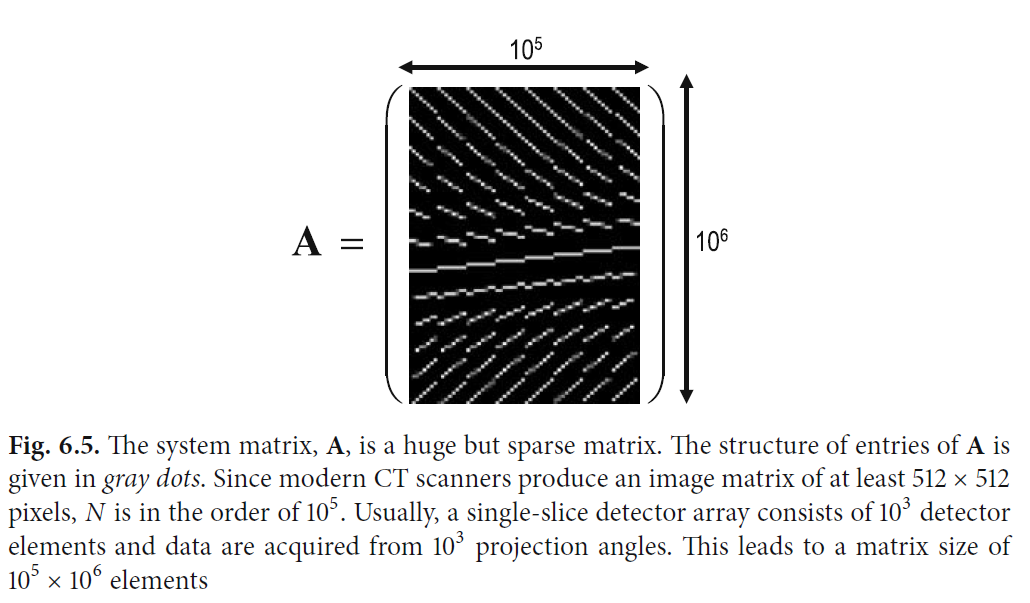
\includegraphics[width=0.4\linewidth,trim={5cm 3cm 5cm 0.5cm},clip]{images/sparsity.png}
 \end{frame}

 \begin{frame}
 \frametitle{SIRT}
 Solve the problem:
 \begin{align}
 \vec{f}^{\ast}=argmin_{\vec{f}}\norm{\vec{p}-\mat{A}\vec{f}}
\end{align}
iteratively using this update step:
 \begin{align}
\vec{f}^{n} = \vec{f}^{(n-1)}+\mat{C}\mat{A}^{T}\mat{R}(\vec{p}-\mat{A}\vec{f}^{(n-1)}),
\end{align}

where $\mat{C}$ and $\mat{R}$ are the diagonal matrices containing the inverse column and row sums of the system matrix respectively.
 \end{frame}

  \begin{frame}
  \frametitle{SIRT}
  \centering
 
\includegraphics[width=0.8\linewidth]{images/sirt.png}
 \end{frame}

 \begin{frame}
 \frametitle{Futhark}
 \begin{itemize}
\item{High level data-parallel, and purely functional array language}
\item{Comes with a heavily optimising ahead-of-time compiler}
\item{Has performed well on several benchmarks}
\item{Hardware-agnostic}
\end{itemize}
 \end{frame}

 \begin{frame}
 \nocite{*}
 \bibliographystyle{plain}
 \bibliography{gpu}
 \end{frame}

\end{document}
